\documentclass[14pt,a4paper]{scrartcl}
%too many packeges
\usepackage[utf8]{inputenc}
\usepackage[english]{babel}
\usepackage{indentfirst}
\usepackage{misccorr}
\usepackage{apacite}
\usepackage{graphicx}
\usepackage[section]{placeins}
\usepackage{float}
\usepackage{tabularx}
\usepackage{color}
\usepackage{fancyhdr}
\usepackage{times}
\usepackage{gensymb}
\usepackage{verbatim}
\usepackage{mathtools}
\usepackage{titlesec}
\usepackage{url}
\usepackage[T1]{fontenc} 
\usepackage{sectsty}
\usepackage{natbib}
\usepackage{makecell}
\usepackage{dsfont}
\usepackage[labelsep=period]{caption}
\usepackage{subcaption}
\usepackage{setspace}
\usepackage{titletoc}
\usepackage{mathrsfs}
\usepackage{circuitikz}
\usepackage[nottoc,notlot,notlof]{tocbibind}
\definecolor{mygray}{gray}{0.4}
\usepackage[top=2.5cm,bottom=2.5cm,right=2.5cm,left=2.5cm,bindingoffset=0cm]{geometry}
\usepackage[colorlinks=true, a4paper=true, pdfstartview=FitV,
linkcolor=black, citecolor=mygray, urlcolor=black]{hyperref}

\DeclareMathOperator*{\argmax}{arg\,max}

%formating routine
\titleformat{\subsection}[block]{\bfseries{\hspace{2em}}}{\thesubsection}{1em}{}
\titleformat{\subsubsection}[block]{\bfseries{\hspace{3em}}}{\thesubsubsection}{1cm}{}
\newcommand{\sectionbreak}{\pagebreak}
\sectionfont{\centering}
\renewcommand{\baselinestretch}{2.0}
\captionsetup{compatibility=false}
\setlength{\parindent}{0.5in}
\setlength{\parskip}{6pt}
\graphicspath{ {images/} }
\linespread{1.25}
\pdfcompresslevel=9

%Macros for numeration
\makeatletter
\renewcommand{\@seccntformat}[1]{%
  \ifcsname prefix@#1\endcsname
    \csname prefix@#1\endcsname
  \else
    \csname the#1\endcsname\quad
  \fi}
\newcommand\prefix@section{Chapter \thesection. }
\makeatother
%Hack for prefixes in toc
\titlecontents{section}[3.5em]{\medskip\bfseries}
{\contentslabel[\color{black}Chapter \thecontentslabel]{4.5em}\enspace}
{\hskip-3em}
{\titlerule*[1.2pc]{.}\contentspage}

\newcommand{\norm}[1]{\left\lVert#1\right\rVert}
\begin{document}

	\begin{titlepage}
		  \begin{center}
		    \large
		    \textbf{The Government of the Russian Federation}
		    
		    \textbf{Federal State Autonomous Educational Institution\\of Higher Professional Education}
		    \vspace{0.25cm}
		    
		   \textbf{National Research University – Higher School of Economics}
		   \vspace{0.25cm}

		   	Faculty of Social Sciences
		    \\School of Psychology\\[1cm]
		    
		    \textbf{Undergraduate Thesis}
		    \\[0.5cm]
		    \textbf{\guillemotleft Neurophysiological Correlates Of Efficient Learning In The Neurofeedback Paradigm \guillemotright}
		    \vfill
		     
			\end{center}

	\newlength{\ML}
	\hfill\begin{minipage}{0.4\textwidth}
	  \textbf{Student group BPS-143}\\[0.3cm]
	  \underline{Minkov V.\,A.} \\
	  \scriptsize{Last name, First name, Middle name}\\\\
	  \large
	  \underline{\hspace{7cm}}
	  \scriptsize{Signature}\\
			\end{minipage}%


	\hfill\begin{minipage}{0.4\textwidth}
	  \textbf{Scientific adviser}\\[0.3cm]
	  \underline{Professor\, PhD} \\
	  \scriptsize{Position, Academic degree}\\\\
	  \large
	  \underline{Ossadtchi A.\,E.} \\
	  \scriptsize{Last, F. M/O.}\\\\
	  \underline{\hspace{7cm}}
	  \scriptsize{Signature}\\
			\end{minipage}

	\hfill\begin{minipage}{0.4\textwidth}
		\textbf{Consultant}\\[0.3cm]
		\underline{Smetanin N.\,V.} \\
		\scriptsize{Last, F. M/O.}\\\\
		\underline{\hspace{7cm}}
		\scriptsize{Signature}\\
			\end{minipage}

	    \vfill
	    \vfill
	    \vfill  

		\begin{center}
		\vfill
		  Moscow, 2018
		\end{center}
	\end{titlepage}


\newpage
\tableofcontents
%Formating routine again
\fancyhf{} 
\renewcommand{\headrulewidth}{0pt} 
\footskip = 30pt
\fancyfoot[R]{\thepage} 
\pagestyle{fancy}
\fancypagestyle{plain}{
  \fancyhf{}
  \renewcommand{\headrulewidth}{0pt}
  \fancyhf[lef,rof]{\thepage}
}
\addtocontents{toc}{\protect\thispagestyle{empty}}

%All party here
\newpage
\section{Introduction}
\label{sec:Introduction}

Operant conditioning is a special way of forming reflexes (involuntary movements in response to a stimulus), that implies reinforcing a reaction that occurs spontaneously, that is, due to the consequences: reinforcement or punishment. The concept of operant conditioning was introduced by Burrhus Frederic Skinner in his book «The Behavior of Organisms» \cite{Jones1939}, although it was first extensively studied by \cite{Thorndike1898} a few decades earlier. There is a number of studies on brain activation evoked by the operant conditioning. A group of brain structures responsible for the operant conditioning is widely recognized as part of the rewarding system – neural network responsible for emotions, incentive salience and learning \cite{Schultz2015}. 

Neurofeedback is a procedure that involves real-time displays of brain activity to reward a subject \cite{Kamiya2011}. According to definition, it appears to be a reinforcement learning process and its efficiency critically depends on the extent to which the feedback signal is matched to the particular subject. Feedback signal latency, color, shape, pitch, timbre, etc. are the ergonomic parameters that may potentially strongly affect the efficiency of learning and the intensity of plastic changes – brain’s ability to change throughout life. Finding the proper ergonomic settings for each particular patient has a potential to boost the efficacy of the neurofeedback therapy and to further prove its usefulness in treating various neurological diseases.

\newpage
\section{Hypothesis}
\label{sec:Hypothesis}

\subsection{Summary}
\label{sec:Hypothesis:Summary}

On the one hand, considering the fact that many animals live without a well developed neocortex, like reptiles and anamniotes, many studies seem to focus on the role of basal ganglia (a group of subcortical structures) in the process of learning. For example, it was suggested that the amygdala, an important part of basal ganglia, plays a chemosensory role and also takes part in the formation of emotions, since the amygdala actually participates in mediating emotional reactions to chemical signals \cite{Martinez-Garcia2010}. Anatomical studies have shown that the amygdala is connected to the olfactory bulb, which affects the perception of sexual pheromones. Although, such results might stress the role of basal ganglia in the process of learning, they do not seem to be absolutely relevant to humans, as they have a more developed neocortex that shares some functions of basal ganglia in the animal brain.

On the other hand, the term «cognitive control» has recently been developed, which includes the function of reinforcement learning \cite{Cockburn2011}. Cognitive control is a collective term describing interrelated processes linked to flexible, purposeful behavior. For example, Ridderinkhof et al. \cite{Ridderinkhof2004} in their review of primate and human studies, along with a meta-analysis of the human functional neuroimaging literature has shown that the medial frontal cortex, or rather its part, anterior cingulate cortex, is believed to be involved in such processes as monitoring the need for increasing cognitive control; behavior correction by sending signals to other cortical structures. Comparing this work to the previous one, we may say that the researchers stress the role of neocortex forgetting about the basal ganglia, which might be insufficient for our research.

As we may see from the works we’ve covered, although the «reward system» and cognitive control are terms that represent different concepts, they are interrelated, because similar structures correlate with their activation, namely the anterior cingulate cortex; different researchers attribute similar functions to both systems; and the reward system, and cognitive control are associated with targeted behavior, and therefore with operant conditioning. Using an integrative approach, suggested by Cockburn and Frank \cite{Cockburn2011}, taking under the consideration both the role of basal ganglia and the role of neocortex, may help to interpret data received from human reward system. For instance, cognitive control theory of beta-wave part may be applied to our research as it attracts our scientific interest.

Why should we integrate these two concepts? The fact is that studies for cognitive control have rich data linking the learning processes with brain rhythms and electroencephalography.

First, it was established that the medial prefrontal cortex generates a high-power theta waves in the conflict of motor tasks. The study by Luu and Tucker \cite{Luu2001} has shown that the mean and lateral oscillations are present for both correct and erroneous answers. When an error occurs, the oscillation of the midline is typed strongly. The initial analysis localizes the oscillation of the midline to the central frontal cortex and lateral oscillations to the sensorimotor cortex. Unfortunately, the study is focused on theta waves and there is no opposition to erroneous answers given. As we have already said, we would prefer to be able to monitor both correct and erroneous answers.

Secondly, the most popular theory of frontal beta waves suggests that the power of this rhythm increases in case of effective performance of the task, and supports the current motor and cognitive state with the help of top-down control. Engel and Fries \cite{Engel2010} have shown that beta activity indicates whether the current sensorimotor or cognitive state is supported. However, just as in the previous study, this one tends to register correct answers only, not paying attention to the wrong ones.

Our main concern was that such complex functions as, for example, the processing of the answer, may not reach the threshold of awareness, but will still have physiological correlates, which Gaal and Lamme have shown in one of their studies \cite{VanGaal2012}.

\subsection{Reinforcement Learning}
\label{sec:Hypothesis:Reinforcement Learning}

\subsubsection{Historical Background}
\label{sec:Hypothesis:Learning Process:Historical Background}

\subsubsection{Modern Concepts Of The Learning Process}
\label{sec:Hypothesis:Learning Process:Modern Concepts Of The Learning Process}

\subsection{Bioelectricity}
\label{sec:Hypothesis:Bioelectricity}

\subsubsection{Definition}
\label{sec:Hypothesis:Bioelectricity:Definition}

Bioelectricity is a general term that is used to encompass electrical potentials and currents occurring within or produced by living organisms. Conversion of chemical energy to electrical energy causes bioelectrical processes. The main difference between electricity in biological and artificial systems is that bioelectrical current is a flow of ions, while standard electricity is a movement of electrons.

\subsubsection{Historical Background}
\label{sec:Hypothesis:Bioelectricity:Historical Background}

\begin{figure}[H]
\centering
\begin{minipage}{.5\textwidth}
  \centering
  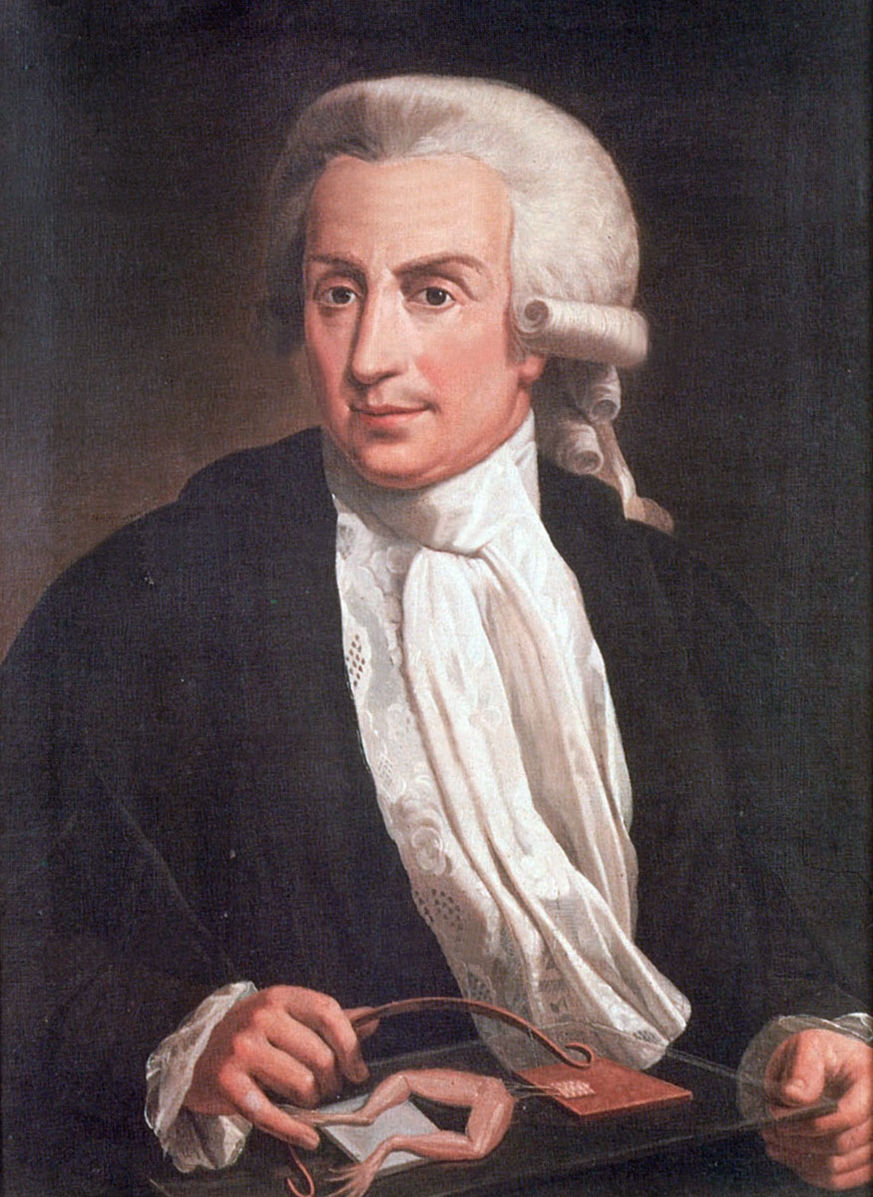
\includegraphics[width=0.5\linewidth]{Galvani}
  \captionof{figure}{Luigi Galvani}\label{fig:Galvani}
\end{minipage}%
\begin{minipage}{.5\textwidth}
  \centering
  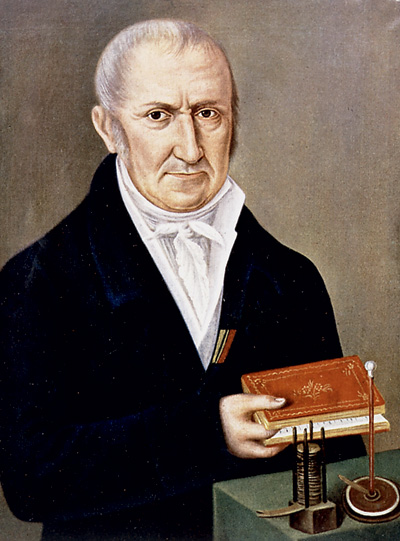
\includegraphics[width=0.5\linewidth]{Volta}
  \captionof{figure}{Alessandro Volta}\label{fig:Volta}
\end{minipage}
\end{figure}

The study of bioelectricity began in 18th century by the physicist \textit{Alessandro Volta} (1745 — 1827) and the physician \textit{Luigi Galvani} (1737 – 1798). Volta created the battery and studied electricity outside of living systems, while Galvani studied electricity in frogs. They both demonstrated that the true explanation of nervous conduction is bioelectricity. However, despite the fact of having common interests, Galvani believed that <<animal electricity>> was fundamentally different from the <<heat electricity>> Volta was studying was studing at the time. We know, that Galvani was wrong, but even nowadays these conflict seems to be reasonable, as manifestation and rules are so different, such as between neuron and galvanic cell, that one might think differently about electricity in artificial and living systems.

\textit{Emil Du Bois-Reymond} was the developer of experimental electrophysiology, the study of the electrical properties of biological cells and tissues. He discovered ways of measuring the tiny electrical currents generated by living tissue. \textit{Julius Bernstein}, a German physiologist, who studied medicine at the University of Berlin with Emil Du Bois-Reymond, hypothesised that nerve and muscle fibers are normally polarized, with positive ions on the outside and negative ions on the inside. According to his theory, the current of living systens results from the reverse of the polarization.

\subsubsection{Ions In Solutions}
\label{sec:Hypothesis:Bioelectricity:Ions In Solutions}

Potentials $\phi$, electric field $E$, electrical forces $F$, current density $J$ and sourses $I_{O}$ are linked together, that is each quantity can be found from the one before. 

An ion is an atom or molecule with a charge. As soon as ions can move, the presence of ions gives a solution electrical conductivity. Consequently, conductivity $\sigma$ is a measure of how many and how easily charges can move. In bioelectrisity, the consentration of $Na^{+}$, $K^{+}$, $Cl^{-}$ are particularly significant, as the higher the concentrations of these ions, the geater the conductivity, if ease of movement is unchanged. 

\begin{figure}[h!]
  \begin{center}
    \begin{circuitikz}
      \draw (0,0) 
      to [generic, o-] (2,0) 
      to [generic, -] (4,0) 
      to [generic, -o] (6,0) 
      node [above = 2em] {Membrane};
      \draw (2,0)
      to [generic, -] (2,2);
      \draw (4,0)
      to [generic, -] (4,2);
      \draw (0,2) 
      to [generic, o-] (2,2)
      to [generic, -, l=Outside (Extracellular Fluid)] (4,2)
      to [generic, -o] (6,2);
      \end{circuitikz}
    \caption{<<Core-conductor model>>}
  \end{center}
\end{figure}

<<Core-conductor model>> is a simple geometrical model, that retains all essential features of a real nerve fiber. Interior and exterior volumes are both conducting solutions. We can use the standart formula to find resistance from resistivity: $R = \frac{\rho_{i}L}{\pi h^{2}}$.

In terms of axial resistance, nerves are not like wires due to large difference in conductivity. 

One gets a transmembrane potential by keeping the negative lead out of the cell and putting the positive lead inside of the cell $V_{trans} = \phi_{inside} - \phi_{outside}$. Axisal potential is got by keeping the negative lead further from the cell body and the positive lead closer to the cell body $V_{axial} = \phi_{b} - \phi_{a}$. 

Assuming that the axial current is uniform it can simply be calculated with Ohm's Law: $I_{x} = \frac{V_{ab}}{R}$.

Assuming that the axial current is uniform from $a$ to $b$, the electric field is change in potential divided by change in possition $E_{x} = \frac{\phi_{a}-\phi_{b}}{l_{a}-l_{b}}$. The electric field $E_{x}$ is a measure of the force $F$ that will be exerted on each of the charged particles. So knowing the electric field gives you some insight that you don't have unless you calculate how much that is.

Once we know the electric field, we can find the axial current density and then the axial current. First, to get the axial current density, we use this expression, and substitute in numbers. The axial current density $J$ in the $X$ direction is equal to the interior conductivity times the electric field $J_{x}=\sigma_{i}E_{x}$ or to the  axial current divided by cross section area $J_{x}=\frac{I}{S}$. 



\subsection{Neurofeedback}
\label{sec:Hypothesis:Neurofeedback}

\textit{\textbf{Biological feedback} (biofeedback, BFB)} is a process in which the subject is presented with some visual representation of their physiological state, as a result of which the subject can somehow manipulate it. The method of \textit{\textbf{neural feedback} (neurofeedback, NFB)} – also known as EEG biofeedback – is a special case of biological feedback, that measures brain waves to generate a signal that can be used as feedback to teach self-regulation of subject's brain function. 

The method of neural feedback has been used since the 1960s and became an effective non-invasive treatment tool for patients with a various disorders, such as epilepsy \cite{Strehl2014,Kotchoubey2001}, attention deficit hyperactivity disorder (ADHD) \cite{Leins2007,Sonuga-Barke2013,Thompson2005}, autistic spectrum disorder (ASD) \cite{Kouijzer2009,Thompson2009}, strokes \cite{Rayegani2014}, tinnitus \cite{Hartmann2014}, emotional disorders \cite{Raymond2005} and posttraumatic stress disorder \cite{Othmer2009}. However, it is not widespread enough, in favor of invasive therapy, because it cannot be accurately established during the use of the neural feedback method, whether the patient is on the mend or not. The judgements can only be made after a while whether the seizures are repeated or not. Or, in extreme cases, introspectively. This problem even has a special name: the «Neurofeedback Inefficiency Problem». With the advent of methods of neurovisualization, it became clear that the effectiveness of training can be associated with the activation in the frontal areas of the cortex of the cerebral hemispheres, what we’ve described above. Therefore, probably today, a method of monitoring the learning process in the paradigm of neural feedback can be found. During the operant conditioning of any rhythm in the neural feedback paradigm, it is necessary to control beta-rhythm activation in the frontal areas during effective training, which is likely to be related to maintaining the current motor or cognitive state associated with effective learning \cite{Engel2010}.

\newpage
\section{Method}
\label{sec:Method}  

\subsection{Summary}
\label{sec:Methods:Summary}

So, in the experiment, the neurofeedback method was used. It was implemented with the help of NFBLab software (nfb-lab.readthedocs.io). Using this method, we decided to train the occipital alpha rhythm of the subject, as it was the easiest one to evoke. The artificial training of this rhythm for healthy people does not lead to any disorders. The aim of the study was to reveal the correlates of effective learning in the frontal beta-rhythm associated with the performance of tasks. The design of the experiment was as follows.

The subjects were trained either with real feedback on their alpha waves discrete power extracted from the P4 electrode or with mock-feedback. During the training they were instructed to sit as still as possible and focus on the visual feedback in the form of a game in which a spacecraft was flying from the earth to the space. Whenever P4 alpha power had a large magnitude, a spacecraft would make a small jump towards the space. The task was to make the spacecraft fly as far away from earth as possible by attempting to up-regulate a subject’s P4 alpha power. Mock feedback was derived from the electroencephalography data recorded from the same subject during one of the previous trials and was thus unrelated to the current value of alpha power.

Each session consisted of 4 experimental trials 10 minutes long each and mock vs real feedback condition trials were randomized.  Note that in this paradigm we did not aim at training alpha but rather attempted to catch the low-level difference between the consistent and inconsistent feedback as it is perceived by the brain.

For each participant we recorded the electroencephalography data for mock and real feedback conditions at 500 Hz sampling rate. The data were then filtered with a band-pass finite impulse response filter in 30 different frequency bands from 1-30 Hz range with 2 Hz bandwidth. The the data was cut to small pieces. The beginning of the piece was considered to be when the reinforcement was presented. The end of the stimuli was 1000 ms later. The data pieces from the two conditions (real and mock feedback) were contrasted using the common spatial pattern procedure. Common spatial pattern is a mathematical technique that separates a multivariate signal into subcomponents with maximum differences in variance between two windows \cite{Koles1990}. It is used in the field of digital signal processing to compare two types of data and to stress the difference between them.

In order to establish the significance of the observed differences we performed non-parametric randomization test to obtain the $p-values$ of null hypothesis of no significant changes between the real and mock feedback conditions \cite{Maris2007}. Next, a correction for the number of false detection rate was applied to the obtained $p-value$ \cite{Benjamini2001}.

To test the effectiveness of the mathematical algorithm described above, we first decided to test the quality of the algorithm on conditions in which the activation is obviously distinguishable: on the eyes-open condition, when the occipital alpha-rhythm is absent, and on the eyes-closed condition, when the alpha rhythm is present.

\subsection{Experimental Design}
\label{sec:Methods:Experimental Design}

\subsection{Data Analysis}
\label{sec:Methods:Data Analysis}

\subsubsection{Common Spatial Pattern}
\label{sec:Methods:Data Analysis:Common Spatial Pattern}

The common spatial pattern (CSP) technique maximizes the difference between two windows $X_{1}$ and $X_{2}$ of the multivariate signal for separating into additive subcomponents (Eq. 1). If $X_{i}$ is a matrix $n_{i} X t_{i}$, where $n_{i}$ – number of channel and $t_{i}$ – number of samples, such a problem can be solved by computing the two covariance matrices (Eq. 2) and the subsequent spectral decomposition of these two matrices (Eq. 3).

The $CSP(X1, X2)$ function used in the following sections gets two windows of the multivariate signal as arguments and returns an eigenvalue corresponding to the analyzed component that should be used in the next statistical test.

\begin{equation}
w = \argmax_{w}{\frac{\left \| wX_{1} \right \|}{\left \| wX_{2} \right \|}}
\end{equation}
\begin{equation}
C_{i} = \frac{X_{i}X^{T}_{i}}{t_{i}}
\end{equation}

\begin{equation}
C^{-1}_{2}C_{1} = PDP^{-1}
\end{equation}


\subsubsection{Tikhonov Regularization}
\label{sec:Methods:Data Analysis:Tikhonov Regularization}

\subsubsection{Nonparametric Statistical Testing Of EEG Data}
\label{sec:Methods:Data Analysis:Nonparametric Statistical Testing Of EEG Data}

\subsubsection{False Discovery Rate Correction}
\label{sec:Methods:Data Analysis:False Discovery Rate Correction}

\newpage
\section{Results}
\label{sec:Results}  

Firstly, our algorithm managed to tell the eyes-open condition from the eyes-closed condition. We found statistically significant components in the alpha band, with occipital localization which definitely corresponds to visual cortex.

Secondly, we applied our algorithm to data received from four experimental electroencephalographic recordings. Although we expected to find the activation in the beta band, with frontal localization which may correspond to the anterior cingulate cortex, which activity contrasts with the real feedback and mock feedback conditions, no statistically significant differences were found.

\newpage
\section{Conclusions}
\label{sec:Conclusions} 

Since we did not find any activation localized in the frontal regions that could have been consistent to the previous studies, it is important to continue the research. In the further study, learning conditions in the neural feedback paradigm should be improved and the optimal design for the selection of the frontal beta-rhythm should be found.

We’re still not certain if the areas related to effective learning may be used to improve the technique of neural feedback, having the ability to monitor therapy in this paradigm and with the accuracy to establish whether this method is suitable for patients.

\newpage
\section*{Acknowledgements}
\label{sec:Acknowledgements}
\addcontentsline{toc}{section}{Acknowledgements}

\newpage
\section*{Appendices}
\label{sec:Appendices}
\addcontentsline{toc}{section}{Appendices}

\newpage
\bibliographystyle{apa}
\bibliography{/Users/basilminkov/Scripts/latex/alpha_feedback/AlphaFeedback.bib}
\end{document}